\documentclass[a4paper,10pt]{article}
\input{/home/frr/UFSC/Pagina/Dropbox/Modelos/Modelo_prova_latex/estilo_prova.tex}

\begin{document}


\professor{Fábio Rodrigues de la Rocha}
\turma{06655}
\codigodisciplina{ARA7546}
\disciplina{Circuitos Digitais}
\data{02/04/2014}
\hlimite{20:20}
\listaexercicios{4}

\begin{center}
\large{\fbox{\mbox{Decodificadores}}}
\end{center}


\questao{Mostre como é possível construir um decodificador de 3 para 8 usando portas lógicas.} Mostre a tabela verdade, equações para cada uma das 4 saídas, simplifique usando mapas K e crie o circuito eletrônico.

\questao{Mostre como é possível criar um decodificador de 4 para 16 utilizando associação de decodificadores 2 para 4.}


\begin{center}
\large{\fbox{\mbox{Multiplexador}}}
\end{center}


\questao{Explique com suas próprias palavras o funcionamento de um multiplexador.}

\questao{Crie um multiplexador de 4 linhas de entrada (mais 2 linhas de entradas especiais) utilizando portas lógicas.} Apresente o as equações, mapas k e o circuito eletrônico.

\questao{Mostre como utilizar um multiplexador para gerar funções booleanas. Exemplifique para a função lógica: $f(A,B,C)=AB+\overline{A}\,\overline{B}+\overline{C}$}

\questao{Mostre como utilizar um multiplexador para gerar funções booleanas. Exemplifique criando as funções lógicas de um decodificador de 2/4.}

\questao{A figura abaixo mostra 2 computadores (A e B) e um monitor de vídeo. Deseja-se comutar o sinal de vídeo ora do computador A, ora do computador B para o monitor.} Sabe-se que o sinal de vídeo é composto por alguns pinos analógicos R,G,e B (que representam um sinal de tensão que representa a intensidade de cada uma dessas cores) e os sinals H e V que são sinais digitais e representam o sincronismo vertical e horizontal (representam a quebra de linha-  H e quebra de tela - V). Vamos assumir que exista um CI chamado MUX que tem os menos pinos que o multiplexador digital 74157. Mostre como usando várias unidades do CI MUX podemos construir um comutador de vídeo para através de um sinal de controle digital, escolhermos qual computador estará ligado ao monitor. PS: O datasheet do 74157 está na página da disciplina.

\begin{figure}[htb]
 \centering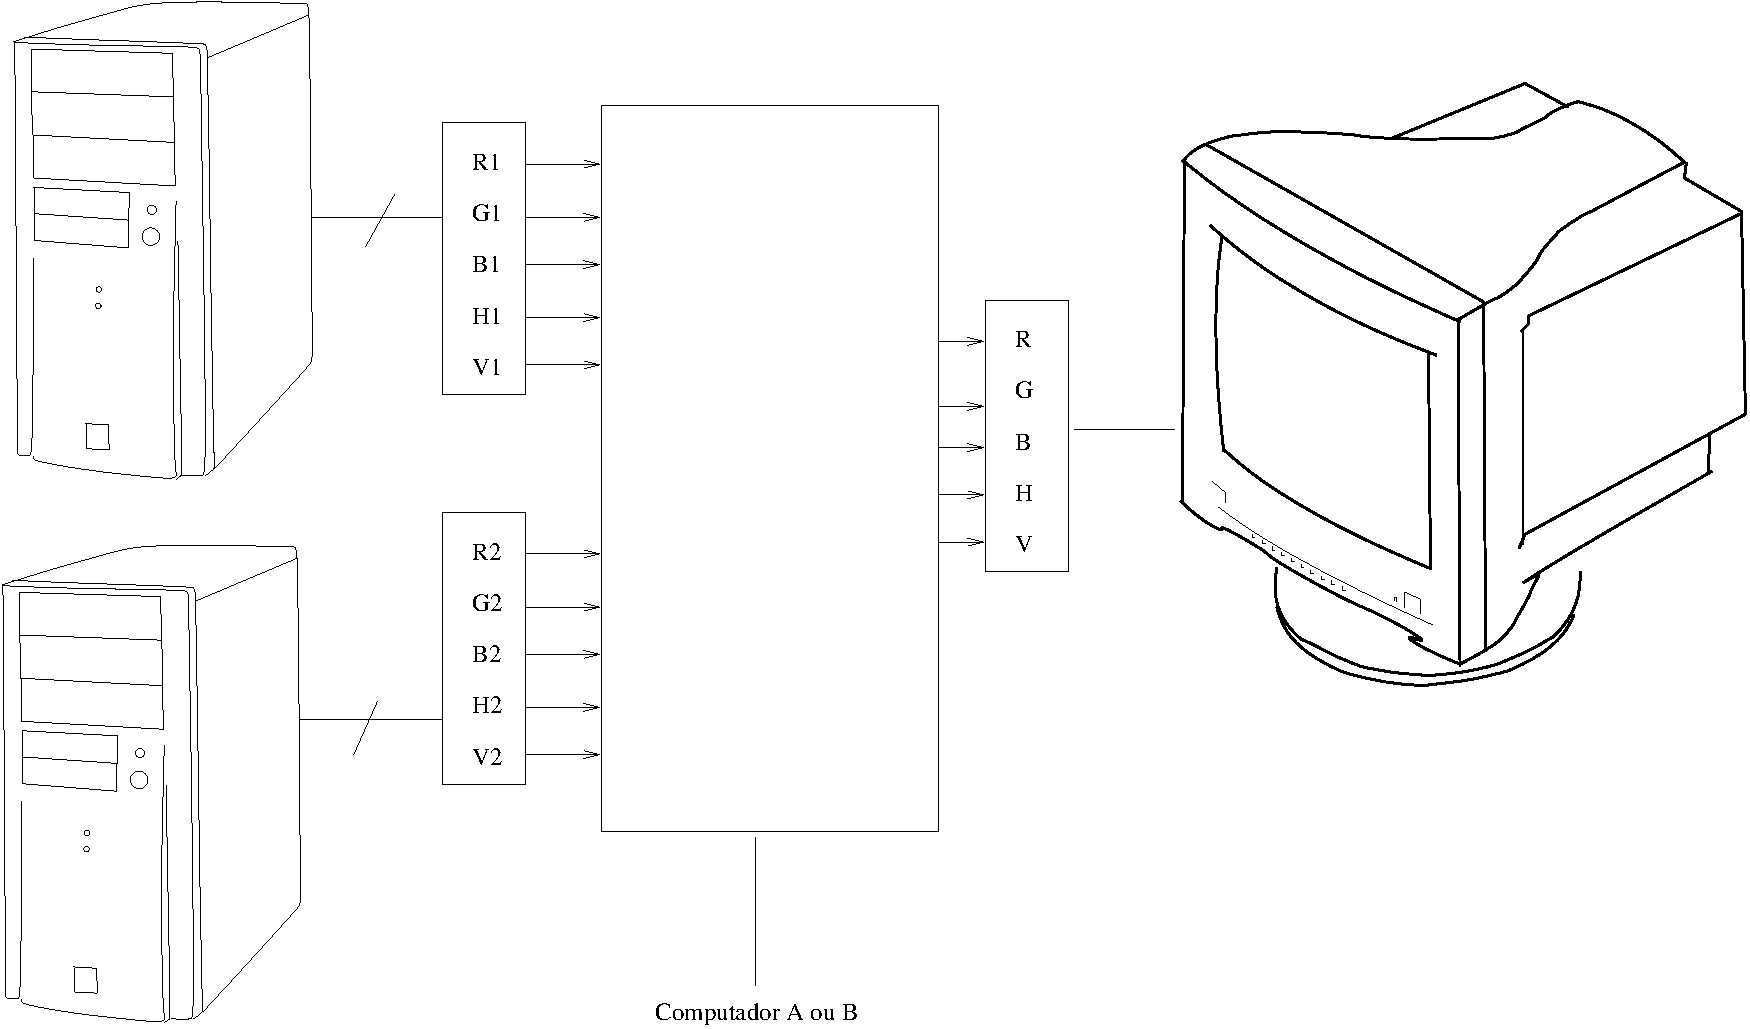
\includegraphics[width=0.4\textwidth]{multiplexador}
\end{figure}


\questao{Implemente as seguintes funções utilizando somente multiplexadores:}
\begin{enumerate}
 \item $f(K,W,O) = \sum{} m(0,3,5,6)$, utilizando um multiplexador de 8 entradas   (74LS151);
 \item $\overline{(\overline{a}\,\overline{\overline{b}\,c})(\overline{\overline{a}\,\overline{b}})(\overline{\overline{a}\,d})} $ utilizando 2 multiplexadores de 8 entradas   Construa um circuito com portas lógicas para selecionar qual dos multiplexadores terá sua saída conectada na saída do circuito.
 \end{enumerate}
 
DICA: CI 74151 - $S_{0}-S_{2}$ -  Entradas de seleção;  $E$ - Entrada de habilitação do CI;  $I_{0}-I_{7}$ Entradas multiplexadas; $Y$ - saída ; $\overline{Y}$ - saída invertida;  
\begin{figure}[htb]
 \centering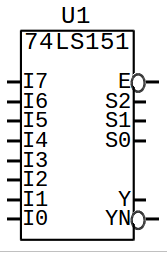
\includegraphics[width=0.1\textwidth]{74151}
\end{figure}




\end{document}